\documentclass{beamer}

\usepackage{amsmath}
\usepackage{amssymb}
\usepackage{mathtools}
%\usepackage{float}
%\usepackage[pdftex]{graphicx}
\usepackage{ngerman}
%\usepackage[T1]{fontnc}
\usepackage[utf8]{inputenc}
%\usepackage{enumerate}
%\usepackage{ifpdf}

\usetheme{Warsaw}

\title{Elektronikpraktikum SS14, Auswertung: Versuchstag 1}
\author{Gruppe 1 \\ Patrick Heuer \\ Benjamin Lotter}
\date{}

\begin{document}
\frame{\titlepage}
%\tableofcontents

\begin{frame}
    \frametitle{Aufgabe 1a}
    \framesubtitle{Schaltplan}
    Hier kommen die Schaltpläne hin
\end{frame}
\begin{frame}
    \frametitle{Aufgabe 1a}
    \framesubtitle{Messreihen}
    Hier kommt die Messreihe hin.
\end{frame}
\begin{frame}
    \frametitle{Aufgabe 1a}
    \framesubtitle{Beobachtungen}
    Hörbares klicken im DMM bei Übergängen 
    \begin{align*}
        \text{Aufwärts:}\quad&
        220mV-240mV\qquad
        280mV-300mV\\
        \text{Abwärts:}\quad&
        60mV-40mV\qquad
        4mV-3mV
    \end{align*}
    \rightarrow 
\end{frame}
\begin{frame}
    \frametitle{Aufgabe 1a}
    \framesubtitle{benis}
    sadf
\end{frame}
%\begin{frame}
%    \frametitle{Aufgabe 1a}
%    \framesubtitle{}
%    \pause
%\end{frame}
%\begin{frame}
%    \frametitle{Aufgabe 1a}
%    \framesubtitle{}
%    \pause
%\end{frame}
%\begin{frame}
%    \frametitle{Aufgabe 1a}
%    \framesubtitle{}
%    \pause
%\end{frame}
%\begin{frame}
%    \frametitle{Aufgabe 1a}
%    \framesubtitle{}
%    \pause
%\end{frame}
%\begin{frame}
%    \frametitle{Aufgabe 1a}
%    \framesubtitle{}
%    \pause
%\end{frame}
%\begin{frame}
%    \frametitle{Aufgabe 1a}
%    \framesubtitle{}
%    \pause
%\end{frame}
%\begin{frame}
%    \frametitle{Aufgabe 1a}
%    \framesubtitle{}
%    \pause
%\end{frame}
%\begin{frame}
%    \frametitle{Aufgabe 1a}
%    \framesubtitle{}
%    \pause
%\end{frame}
%\begin{frame}
%    \frametitle{Aufgabe 1a}
%    \framesubtitle{}
%    \pause
%\end{frame}
%\begin{frame}
%    \frametitle{Aufgabe 1a}
%    \framesubtitle{}
%    \pause
%\end{frame}
%\begin{frame}
%    \frametitle{Aufgabe 1a}
%    \framesubtitle{}
%    \pause
%\end{frame}
%\begin{frame}
%    \frametitle{Aufgabe 1a}
%    \framesubtitle{}
%    \pause
%\end{frame}
%\begin{frame}
%    \frametitle{Aufgabe 1a}
%    \framesubtitle{}
%    \pause
%\end{frame}
%\begin{frame}
%    \frametitle{Aufgabe 1a}
%    \framesubtitle{}
%    \pause
%\end{frame}
%\begin{frame}
%    \frametitle{Aufgabe 1a}
%    \framesubtitle{}
%    \pause
%\end{frame}
%\begin{frame}
%    \frametitle{Aufgabe 1a}
%    \framesubtitle{}
%    \pause
%\end{frame}
%\begin{frame}
%    \frametitle{Aufgabe 1a}
%    \framesubtitle{}
%    \pause
%\end{frame}
%\begin{frame}
%    \frametitle{Aufgabe 1a}
%    \framesubtitle{}
%    \pause
%\end{frame}
%\begin{frame}
%    \frametitle{Aufgabe 1a}
%    \framesubtitle{}
%    \pause
%\end{frame}
%\begin{frame}
%    \frametitle{Aufgabe 1a}
%    \framesubtitle{}
%    \pause
%\end{frame}
%\begin{frame}
%    \frametitle{Aufgabe 1a}
%    \framesubtitle{}
%    \pause
%\end{frame}
%\begin{frame}
%    \frametitle{Aufgabe 1a}
%    \framesubtitle{}
%    \pause
%\end{frame}

\begin{frame}
\frametitle{Aufgabe 1b}
\framesubtitle{}
    \begin{itemize}
        \item Der Einschaltevorgang der Geräte am Messaufbau kann die Messung
    beeinflussen.
        \item Untersuchung des Einflusses auf eine Gleichstrommessung
    \end{itemize}
\end{frame}
\begin{frame}
\frametitle{Aufgabe 1b}
\framesubtitle{1: Messungen}
\begin{figure}[H]
\begin{center}
    \fbox{
        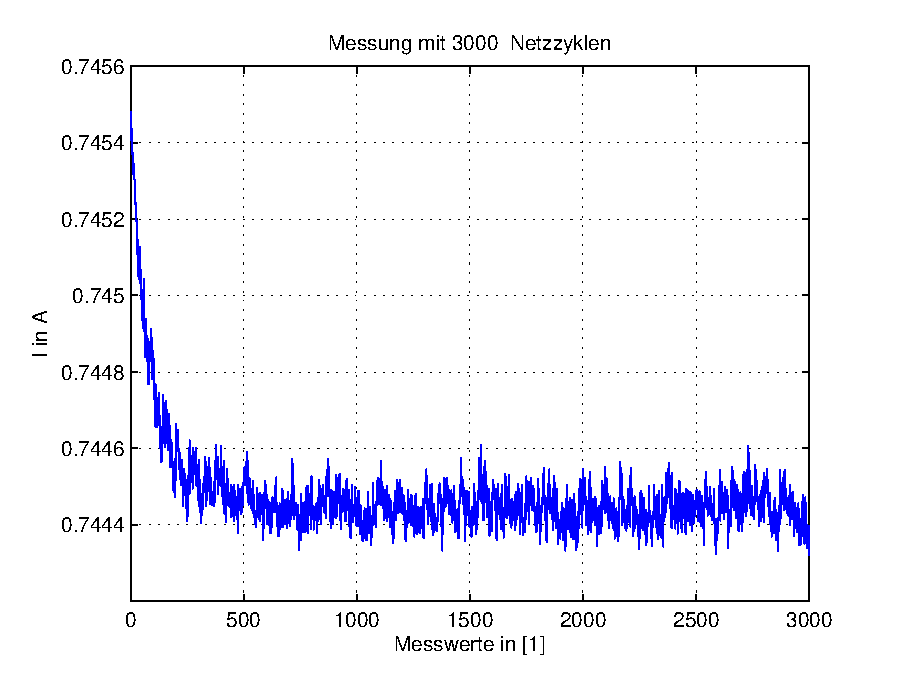
\includegraphics[scale=0.60]{./img/1b13000.eps}
    }
    \caption{Graph 1}
\end{center}
\end{figure}
\end{frame}

\begin{frame}
\frametitle{Aufgabe 1b}
\framesubtitle{1: Messungen}
\begin{figure}[H]
\begin{center}
    \fbox{
        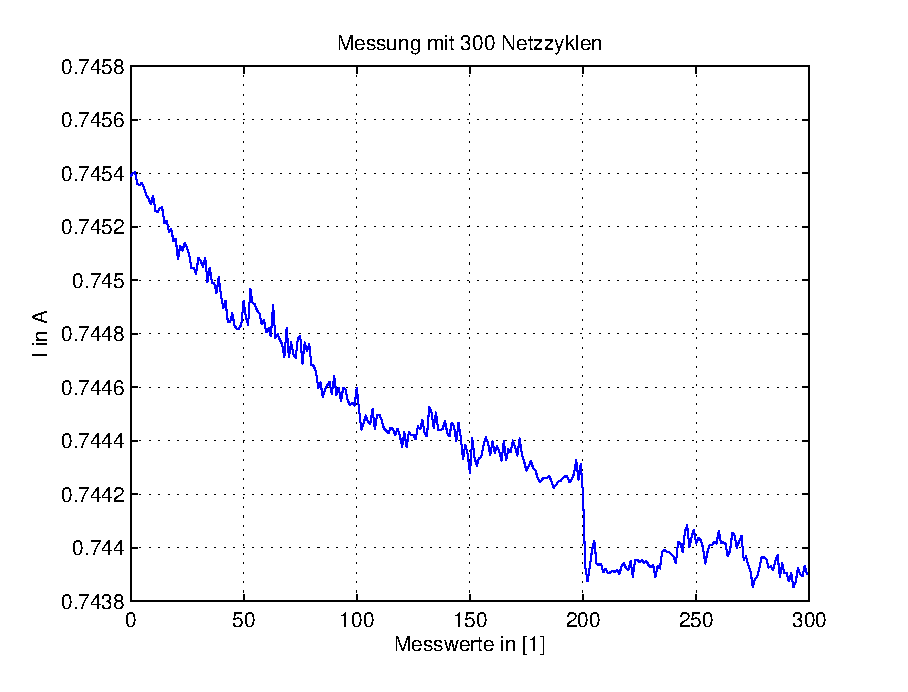
\includegraphics[scale=0.60]{./img/1b1300.eps}
    }
    \caption{Graph 2}
\end{center}
\end{figure}
\end{frame}
\begin{frame}
\frametitle{Aufgabe 1b}
\framesubtitle{Ergebnis}
    Man betrachtet:
    \begin{itemize}
        \item Starker Abfall der Stromstärke von $0-200$
        \item Annährung and den Endwert von $200-500$ in Graph $1$
        \item Sprung auf den Endwert bei $200$ in Graph $2$
    \end{itemize}
    Mögliche Erklärung:
     \begin{itemize}
         \item Bauteile des Geräts müssen sich erst aufwärmen oder einschwingen
         \item Bestimmte Bauteile funktionieren erst ab einer bestimmten
         Temperatur (Sprung in Graph $2$)
     \end{itemize}
    Sofortige Messung nach Einschalten des Geräts liefert keine verlässlichen
    Werte! \\
    Empfehlung des Herstellers: Gerät $30$ Minuten warmlaufen lassen
\end{frame}
\begin{frame}
\frametitle{Aufgabe 1b}
\begin{itemize}
    \item Die Wahl der Integrationszeit kann die Messung beeinflussen.
    \item Der Einfluss der Integrationszeit wurde durch verschiedene
    Netzzyklenzahlen und freie Zeiteinstellung getestet.
\end{itemize}
\end{frame}
\begin{frame}
\frametitle{Aufgabe 1b}
\framesubtitle{2:Messungen}
\begin{tabular}{c|c c c c}
    NPLC   & Maximum    & Minimum    & Mittelwert  &Standardabweichung \\
    \hline
    0,006  & 0,201529   & 0,19882    & 0,20011369  &5,69E-04\\
    0,02   & 0,201495   & 0,198794   & 0,200125373 &5,95E-04\\
    0,06   & 0,201637   & 0,198639   & 0,20012612  &7,70E-04\\
    0,2    & 0,201453   & 0,198895   & 0,200099427 &6,00E-04\\
    1      & 0,200122   & 0,200035   & 0,200076633 &1,54E-05\\
    10     & 0,20006    & 0,199953   & 0,199991067 &2,57E-05
\end{tabular}
\end{frame}
\begin{frame}
\frametitle{Aufgabe 1b}
\framesubtitle{2: Ergebnis}
     Je größer die Standardabweichung, desto mehr liegen Minima und Maxima
     voneinander entfernt $\rightarrow$ mehr Rauschen
     \begin{itemize}
         \item Größte Standardabweichung bei $0.6$ NPLC
         \item Kleinste Standardabweichung bei $10$ NPLC
     \end{itemize}
     $\rightarrow$ Beim Mitteln über Teilzyklen hebt sich das Rauschen nicht
     auf \\
     $\rightarrow$ Beim Mitteln über ganzzahlige Netzzyklen wird das Rauschen
     herausgefiltert \\
     $\rightarrow$ Erhöhung der ganzzahligen Netzzyklen verbessert die
     Genauigkeit
\end{frame}
\begin{frame}
\frametitle{Aufabe 1b}
\framesubtitle{3:Messungen}
\begin{tabular}{c|c c c c}
    NPLC   & Maximum    & Minimum    & Mittelwert  &Standardabweichung \\
    \hline
    0,006  & 0,201529   & 0,19882    & 0,20011369  &5,69E-04\\
    0,02   & 0,201495   & 0,198794   & 0,200125373 &5,95E-04\\
    0,06   & 0,201637   & 0,198639   & 0,20012612  &7,70E-04\\
    0,2    & 0,201453   & 0,198895   & 0,200099427 &6,00E-04\\
    1      & 0,200122   & 0,200035   & 0,200076633 &1,54E-05\\
    10     & 0,20006    & 0,199953   & 0,199991067 &2,57E-05\\
    \hline
    freie Int.& & & &\\
    \hline
    25 ms  & 0,200182   & 0,199796   & 0,19999138  &1,16E-04
\end{tabular}
\end{frame}
\begin{frame}
\frametitle{Aufgabe 1b}
\framesubtitle{3: Ergebnis} 
    Mitteln über eine frei gewählte Zeit ist ungenauer als vielfache NPLCs. \\
    $\rightarrow$ Netzzyklen werden nicht exakt abgeschlossen, Rauschen wird
    nicht vollständig weggehoben

    Wie soll gemittelt werden?
    \begin{itemize}
        \item Teilzyklen: erhöht Rauschen aber verkürzt Messzeit $\rightarrow$
        nur bei sehr vielen Messreihen
        \item vielfache NPCLs: verringert Rauschen aber längere Messzeit
        \item freie Zeit: Nur wenn freie Integrationszeit notwendig
    \end{itemize}
\end{frame}



\section{Analog-zu-Digital-Wandler (ADC)} % (fold)
\label{sec:Analog-zu-Digital-Wandler_(ADC}

\subsection{Erster Funktionstest} % (fold)
\label{sub:Erster Funktionstest}
\begin{frame}
\frametitle{Testsignalschaltung}
\framesubtitle{}
\begin{columns}[c]
    \column{0.65\textwidth}
         \begin{block}{$U_{in}$}
             \begin{itemize}
                \item $U_{in}$ liegt an Tiefpass:
                    \begin{equation*}
                        U_{in} = \frac{1}{\sqrt{\left(1+(R 2 \pi f
                        C)^2\right)}}\cdot U_{Fg} = 0.892V
                    \end{equation*}
                     für $f = 777Hz$,$U_{Fg} = 1V$
             \end{itemize}
         \end{block}
    \column{0.4\textwidth}
        \begin{figure}[H]
        \begin{center}
                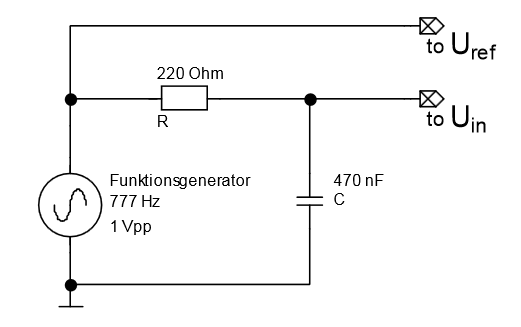
\includegraphics[scale=0.3]{./img/schaltung/testsignal.png}
        \end{center}
        \end{figure}
        \begin{figure}[H]
        \begin{center}
                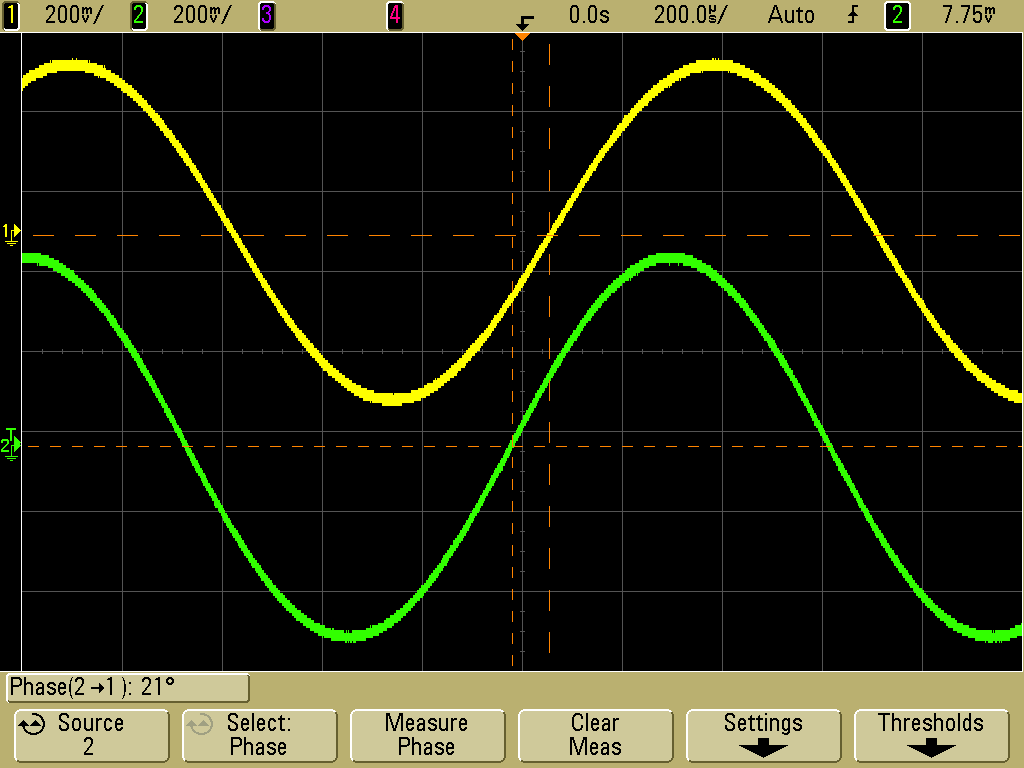
\includegraphics[scale=0.1]{./img/oszi/scope_21.png}
        \end{center}
        \end{figure}
        
        
\end{columns}

\end{frame}

\begin{frame}
\frametitle{Testsignalschaltung}
\framesubtitle{}
\begin{columns}[c]
    \column{0.65\textwidth}
         \begin{block}{Phase}
                 \begin{itemize}
                     \item Theoretische Phasenverschiebung:
                         \begin{equation*}
                             \varphi_{Th} = -\arctan{\left(2\pi f C R\right)} = 26.78^{\circ} 
                         \end{equation*}
                             für $f = 777Hz$
                    \item Gemessene Phasenverschiebung:
                        \begin{equation*}
                            \varphi_{Ge} = 21^{\circ}
                        \end{equation*}
                    \item
                        Mit $R_{Poti} = 6.96k\Omega$ bei maximalem $U_{out}$
                        ergibt sich eine Phasenverschiebung
                        \begin{equation*}
                            \varphi = 17.71^{\circ}
                        \end{equation*}
                 \end{itemize}
         \end{block}
    \column{0.4\textwidth}
        \begin{figure}[H]
        \begin{center}
                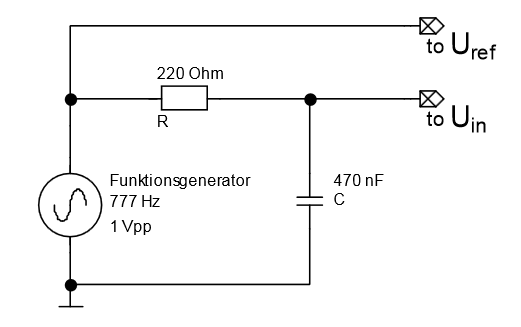
\includegraphics[scale=0.3]{./img/schaltung/testsignal.png}
        \end{center}
        \end{figure}
        \begin{figure}[H]
        \begin{center}
                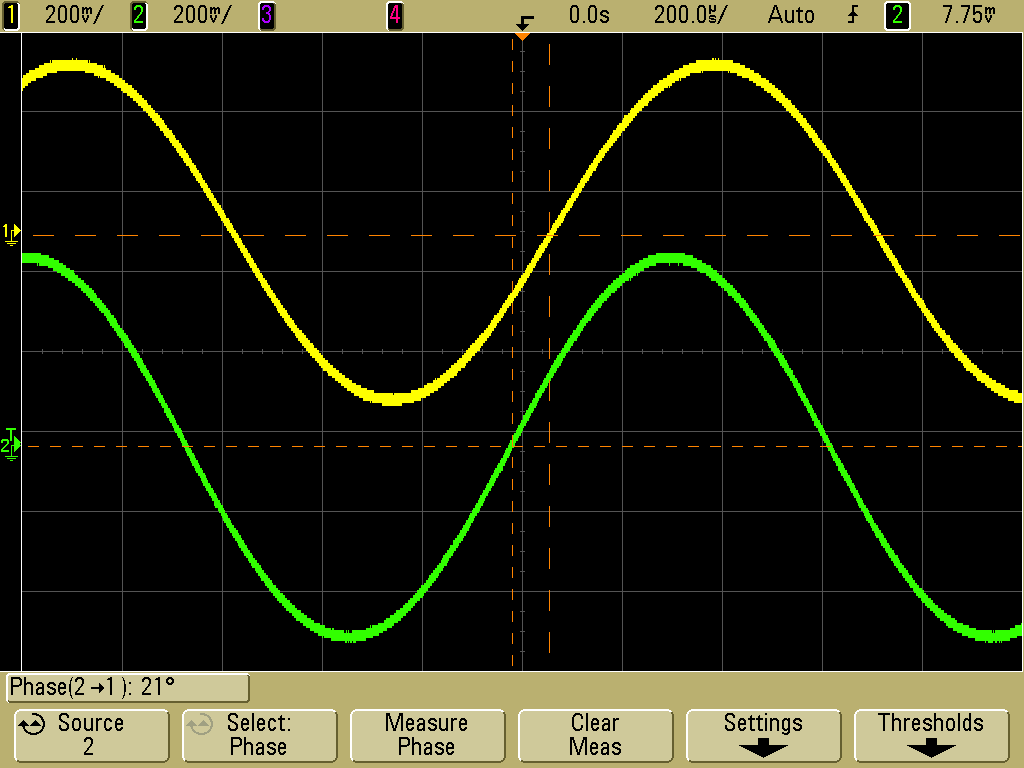
\includegraphics[scale=0.1]{./img/oszi/scope_21.png}
        \end{center}
        \end{figure}
\end{columns}
\end{frame}

\begin{frame}
    \frametitle{Messung}
    \framesubtitle{}
     \begin{figure}[H]
     \begin{center}
             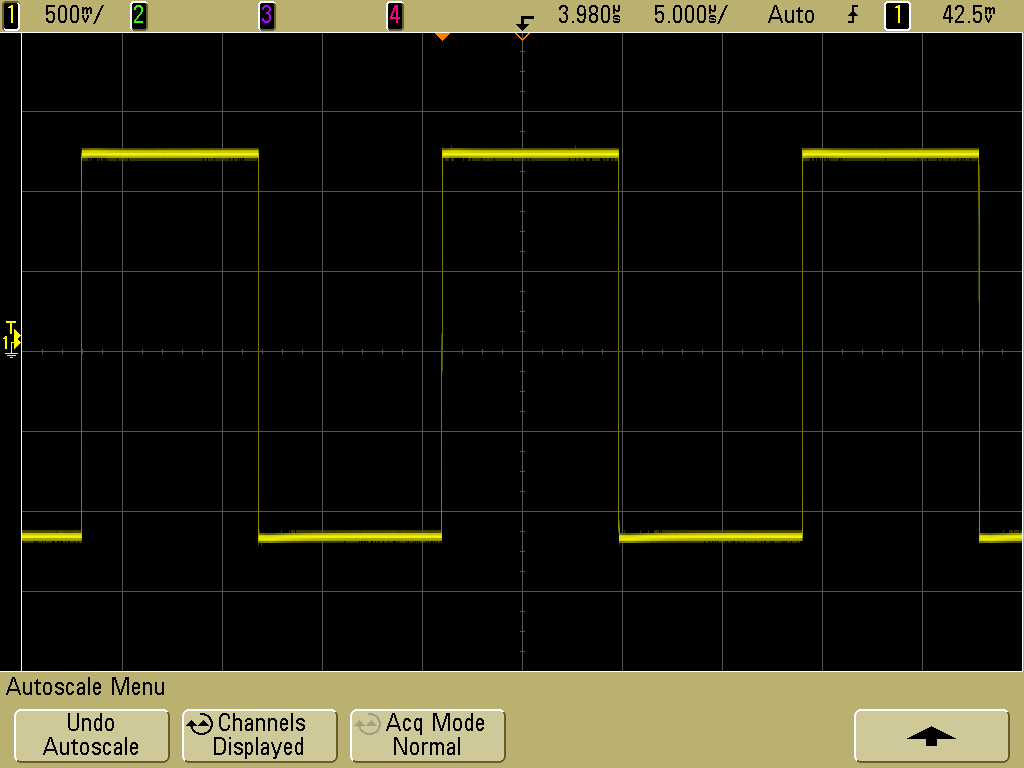
\includegraphics[scale=0.2]{./img/oszi/scope_18.png}
     \end{center}
     \caption{$U_{in}$ und $U_{ref}$ Phasenverschoben}
     \end{figure}
\end{frame}
\begin{frame}
    \frametitle{Messung}
    \framesubtitle{}
    \begin{figure}[H]
    \begin{center}
            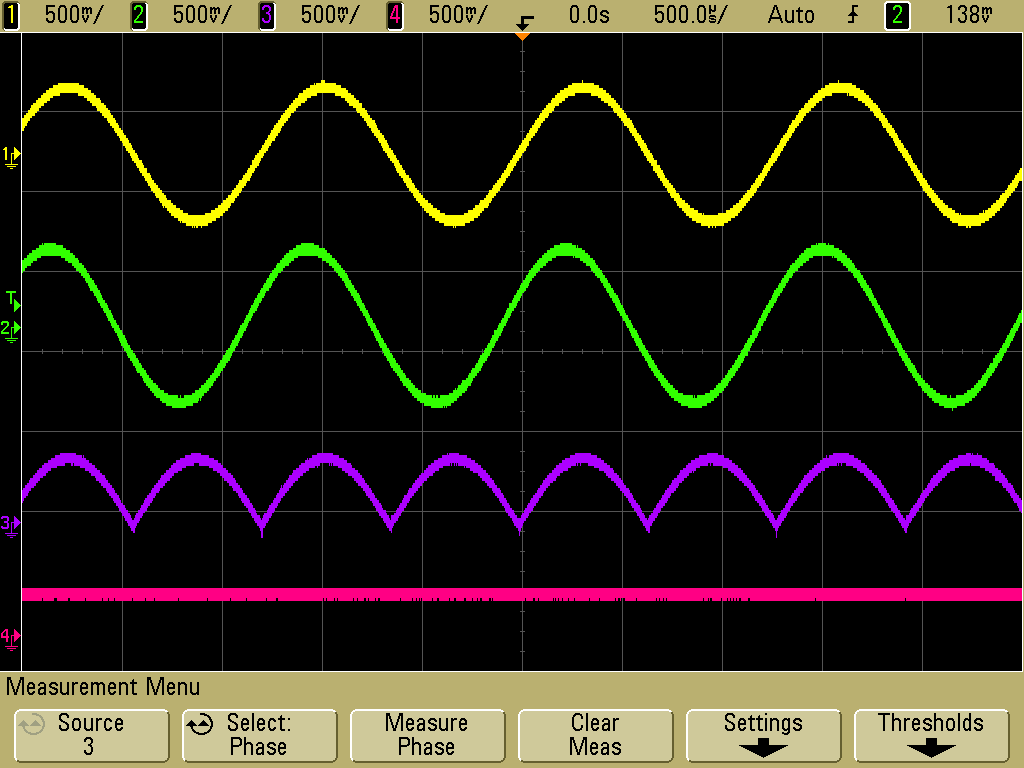
\includegraphics[scale=0.2]{./img/oszi/scope_17.png}
    \end{center}
     \caption{$U_{in}$ und $U_{ref}$ gleichphasig}
    \end{figure}
\end{frame}
% subsection Erster Funktionstest (end)

\subsection{Übertragung eines Lichtsignals} % (fold)
\label{sub:Übertragung eines Lichtsignals}
\begin{frame}
    \frametitle{Übertragung eines Lichtsignals}
    \framesubtitle{}
     \begin{columns}[c]
         \column{0.6\textwidth}
        \begin{block}{Ziel:}
             \begin{itemize}
                 \item Filterung der Störungen durch
                 \begin{itemize}
                     \item Lampen
                     \item Tageslicht
                 \end{itemize}
             \end{itemize}
        \end{block}
        \begin{block}{Versuch}
            \begin{itemize}
                \item moduliere LED-Signal mit $777Hz$ Spannung
                \item gebe Modulationsfrequenz als Referenzfrequenz weiter
                \item benutze L-I-Verstärker um $777Hz$ herauszufiltern
            \end{itemize}
        \end{block}
         \column{0.4\textwidth}
         \begin{figure}[H]
         \begin{center}
                 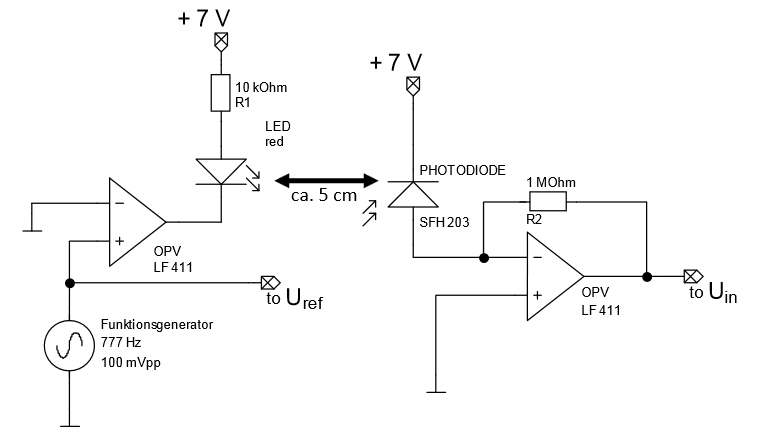
\includegraphics[scale=0.25]{./img/schaltung/optisch.png}
         \end{center}
         \end{figure}
     \end{columns}
\end{frame}

\begin{frame}
    \frametitle{Vergleich mit/ohne Abdeckung}
    \framesubtitle{}
    \begin{columns}[c]
        \column{0.5\textwidth}
        \begin{figure}[H]
        \begin{center}
                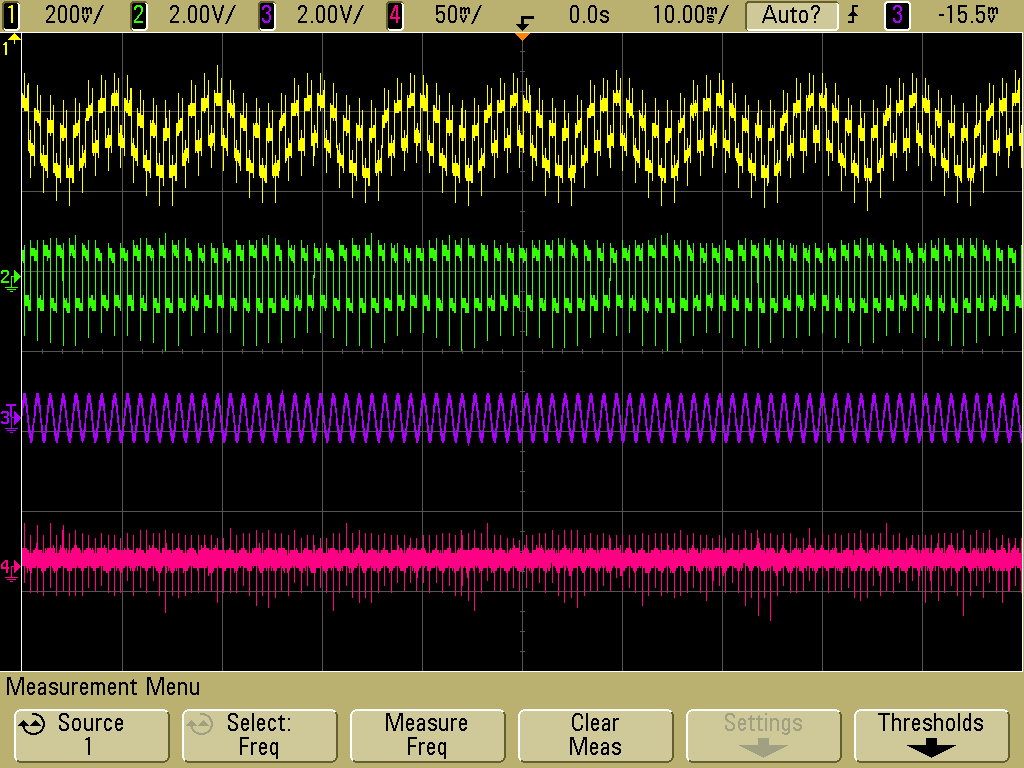
\includegraphics[scale=0.15]{./img/oszi/scope_23.png}
        \end{center}
        \caption{Ohne Abdeckung}
        \end{figure}
        \column{0.5\textwidth}
        \begin{figure}[H]
        \begin{center}
                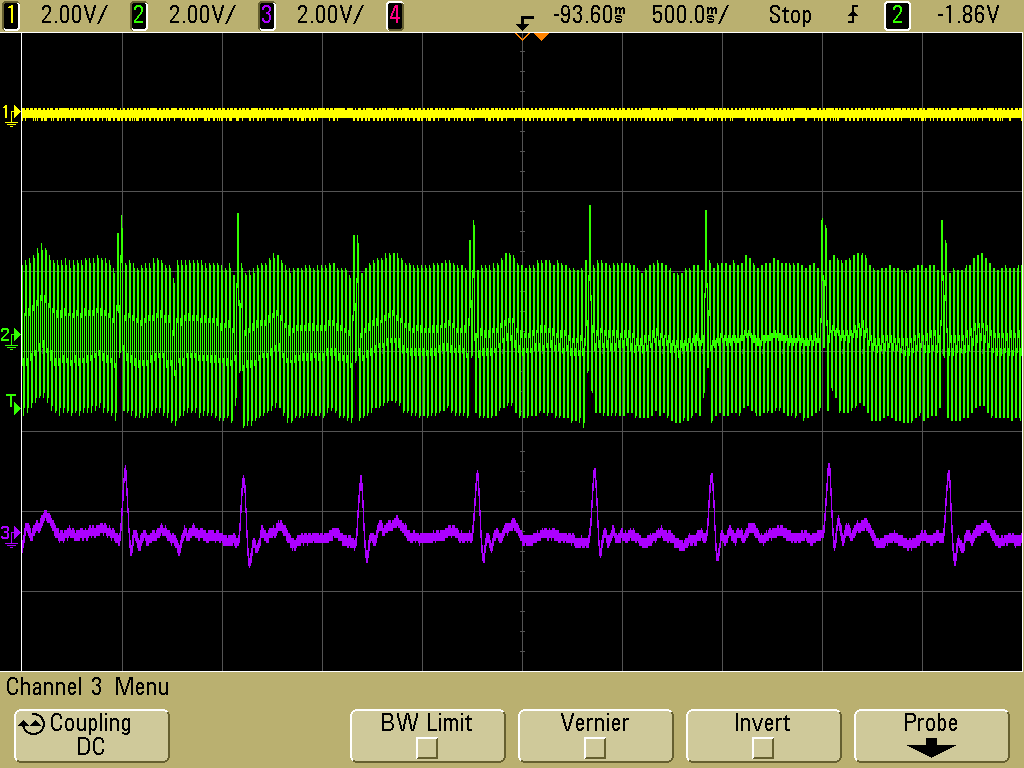
\includegraphics[scale=0.15]{./img/oszi/scope_22.png}
        \end{center}
        \caption{Mit Abdeckung}
        \end{figure}
    \end{columns}
        \begin{block}{}
            Ausgangssignal bleibt konstant auf $52.6mV$ $\rightarrow$ Schaltung
            filtert Störsignale heraus
        \end{block}
\end{frame}
% subsection Übertragung eines Lichtsignals (end)

% section Analog-zu-Digital-Wandler (ADC (end)

\section{Differenzverstärker} % (fold)
\label{sec:Differenzverstärker}
\begin{frame}
    \frametitle{Differenzverstärker}
    \framesubtitle{}
    \begin{block}{Ziel:}
        Verstärkung sehr kleiner Potentialunterschiede $\Delta V \approx 10\mu
        V$ \\ $\rightarrow$ Differenzverstärker
    \end{block}
    \pause
    \begin{figure}[H]
    \begin{center}
            \includegraphics[scale=0.2]{./img/schaltung/difver_1.png}
    \end{center}
    \end{figure}
\end{frame}
\begin{frame}
    \frametitle{Differenzverstärker}
    \framesubtitle{}
    
\end{frame}

% section Differenzverstärker (end)

\begin{frame}
\frametitle{Aufgabe 4}
\framesubtitle{}
    \begin{itemize}
        \item Durch kompliziertere Schaltungen können schärfere
        Frequenztrennungen erreicht werden
        \item Beim Tiefpass wurde fälschlicherweise eine Spule mit $L=100mH$
        verwendet
    \end{itemize}
\end{frame}
\begin{frame}
\frametitle{Aufgabe 4}
\framesubtitle{Tiefpass 2. Ordnung}
\begin{figure}[H]
\begin{center}
        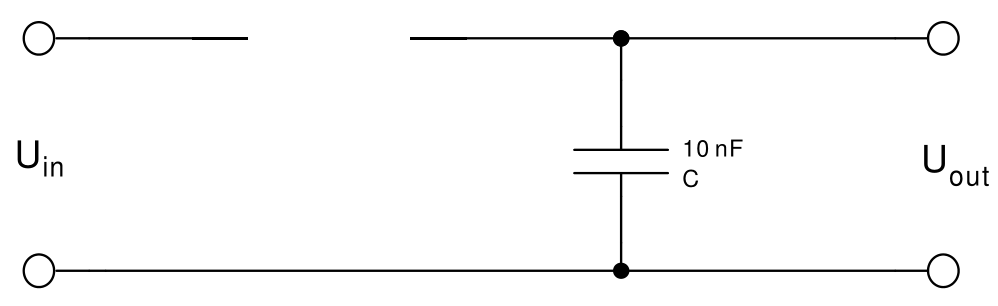
\includegraphics[scale=0.2]{./img/4a_tiefpass_1.png}
\end{center}
\end{figure}
\end{frame}
\begin{frame}
\frametitle{Aufgabe 4}
\framesubtitle{Tiefpass 2.Ordnung}
\begin{figure}[H]
\begin{center}
        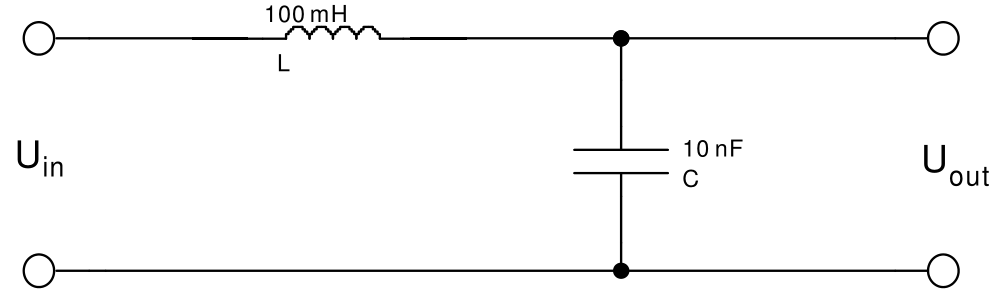
\includegraphics[scale=0.2]{./img/4a_tiefpass_2.png}
\end{center}
\end{figure}
\begin{itemize}
    \item Einbau von Spule
    \item Erwarteter Verlauf
\end{itemize}
\begin{equation*}
    \frac{U_{out}}{U_{in}} = \frac{1}{1-\omega^2 L C}
\end{equation*}
\end{frame}
\begin{frame}
\frametitle{Aufgabe 4}
\framesubtitle{Tiefpass Bode-Diagram}
    \begin{figure}[H]
    \begin{center}
            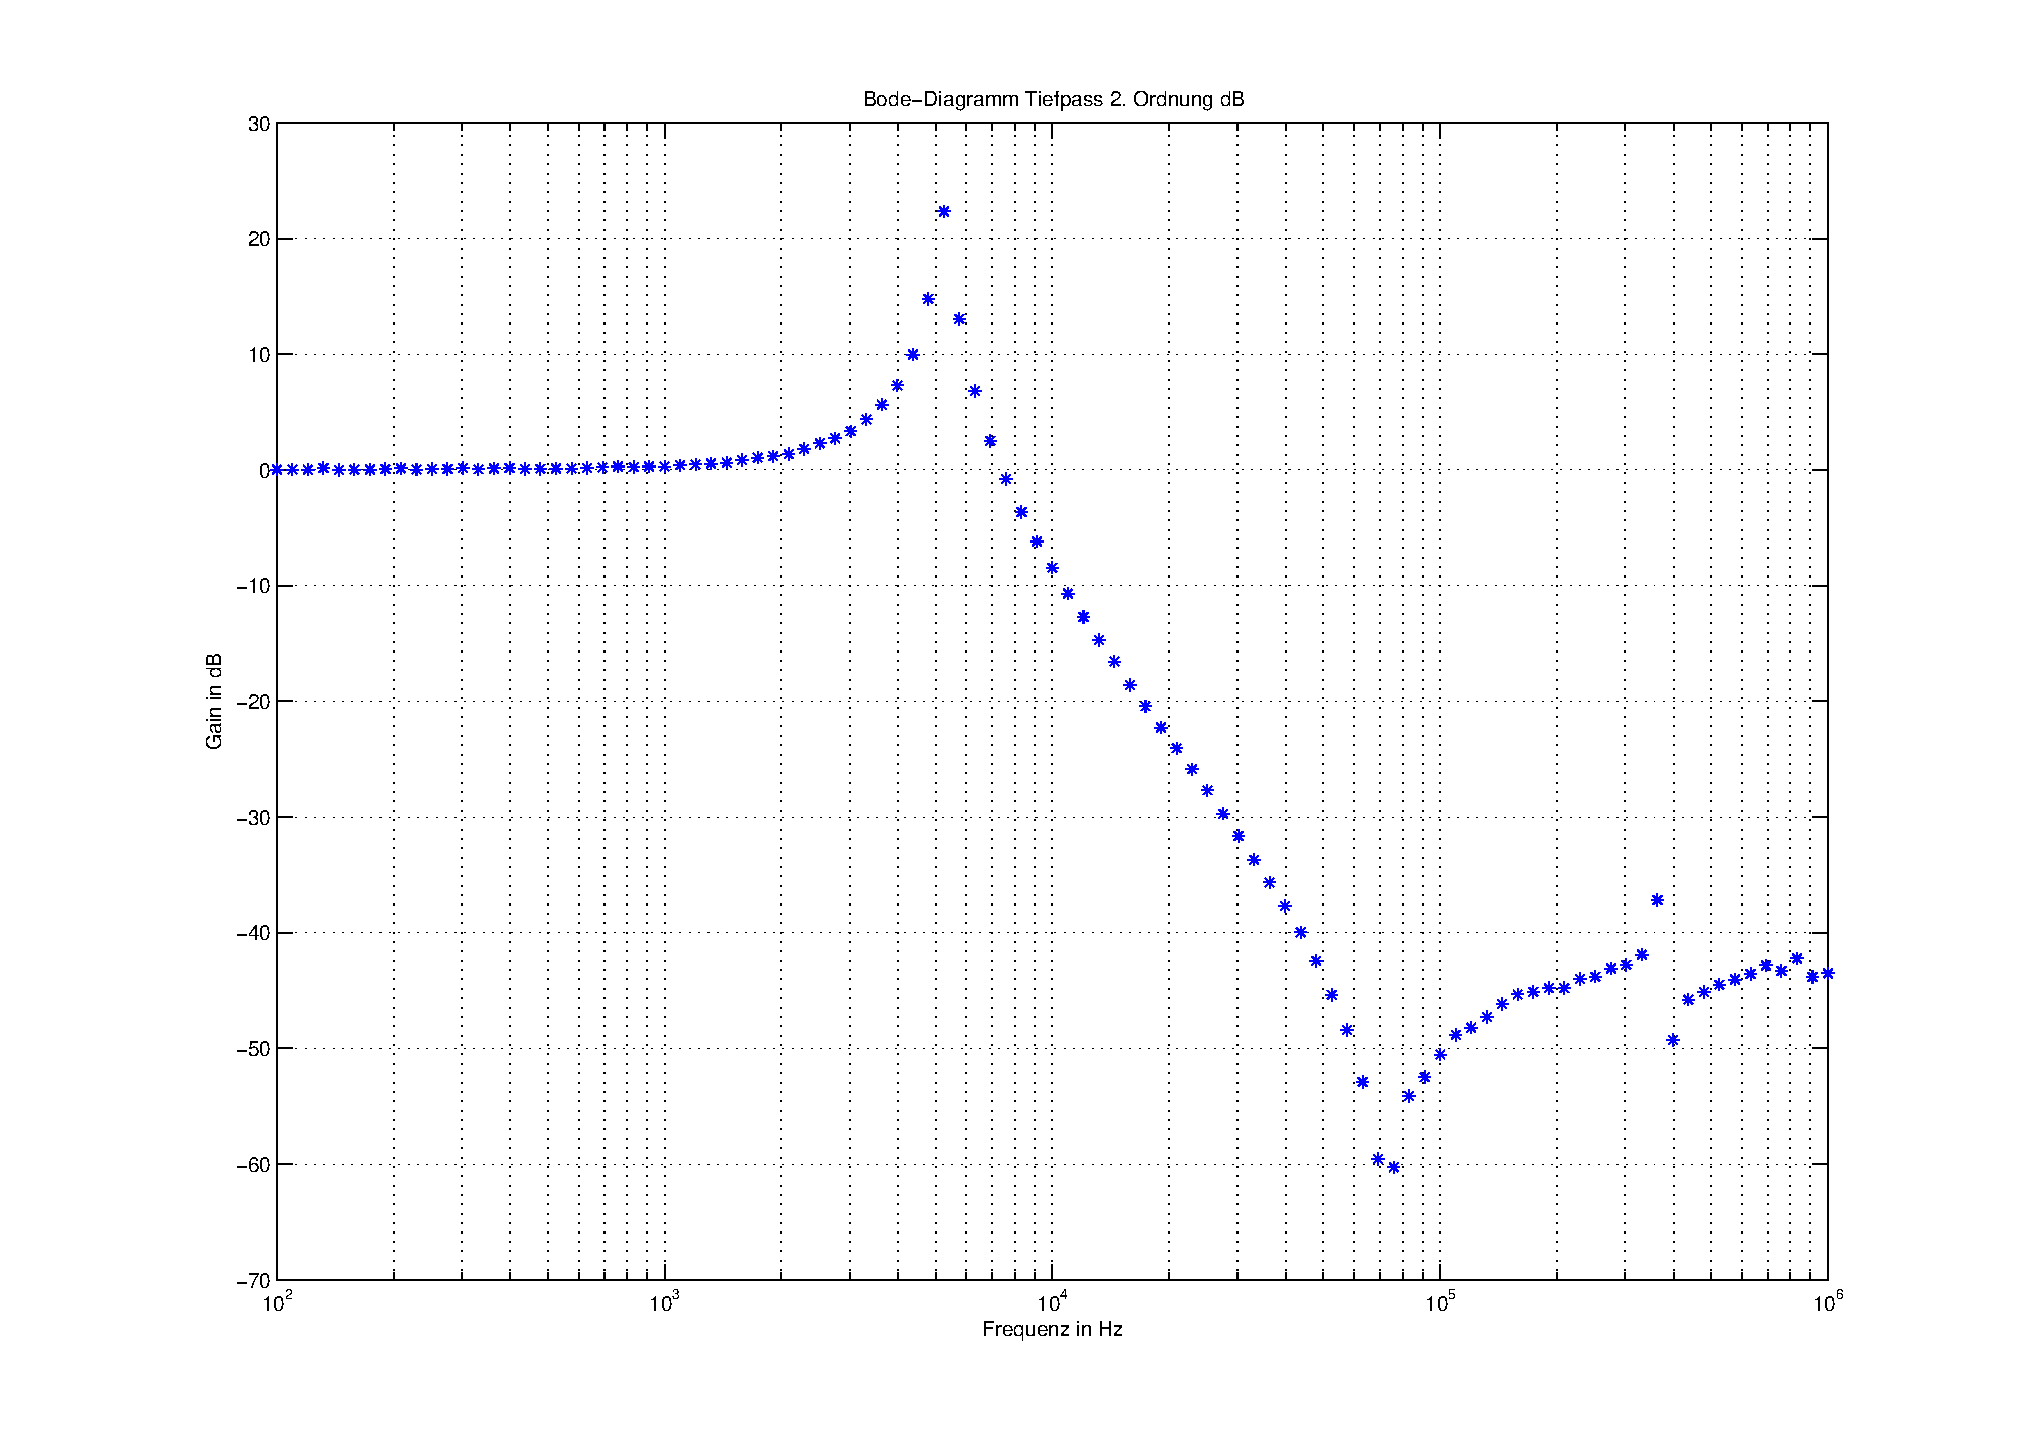
\includegraphics[scale=0.50]{./img/4a_bode_tief_dB.eps}
    \end{center}
    \end{figure}  
\begin{itemize}
    \item Unerwünschte Asymptote bei $\omega = \sqrt{\frac{1}{LC}}$
    \item Schwinkreis ohne Dämpfung
\end{itemize}
\end{frame}
\begin{frame}
    \frametitle{Aufgabe 4}
    \framesubtitle{Tiefpass mit Widerstand}
     %\begin{figure}[H]
     %\begin{center}
     %        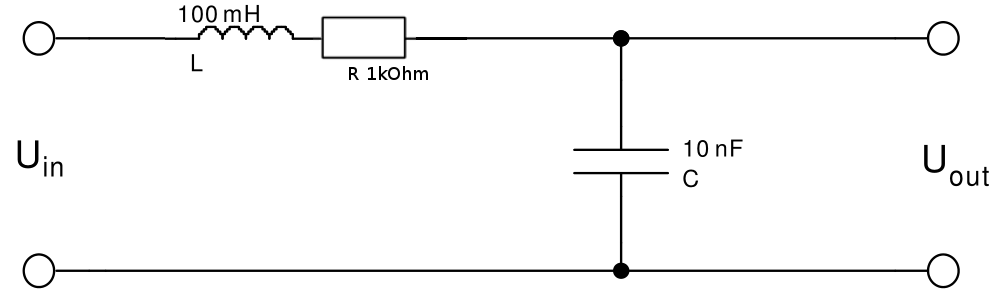
\includegraphics[scale=0.2]{4a_tiefpass_3.png}
     %\end{center}
     %\end{figure} 
     \begin{itemize}
        \item Zusätzlicher Widerstand
         \item Erwarteter Verlauf
     \end{itemize}
     \begin{equation*}
         \frac{U_{out}}{U_{in}}
         =
         \frac{Z_C}{Z_C + Z_L + R}
         =
         \frac{1}{\sqrt{\omega^4 L^2 C^2 + \omega^2 R^2 C^2 - 2 \omega^2 LC + 1}}
     \end{equation*}
\end{frame}
\begin{frame}
    \frametitle{Aufgabe 4}
    \framesubtitle{Tiefpass mit Widerstand}
     \begin{figure}[H]
     \begin{center}
             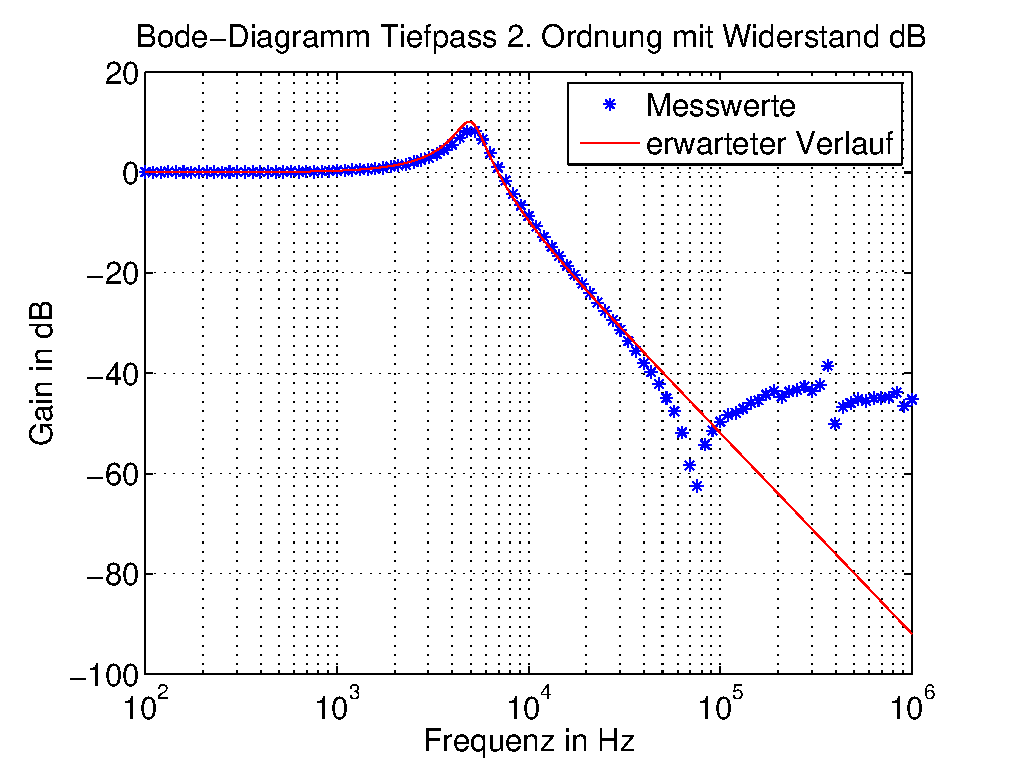
\includegraphics[scale=0.45]{./img/4a_bode_tief_dB_W.eps}
     \end{center}
     \end{figure}
     \begin{itemize}
        \item keine Asymptote
         \item Peak vor Abfall ist deutlich kleiner
         \item $R$ dämpft den Schwingkreis
     \end{itemize}
\end{frame}
\begin{frame}
    \frametitle{Aufgabe 4}
    \framesubtitle{Sperrkreisfilter}
    \begin{figure}[H]
    \begin{center}
            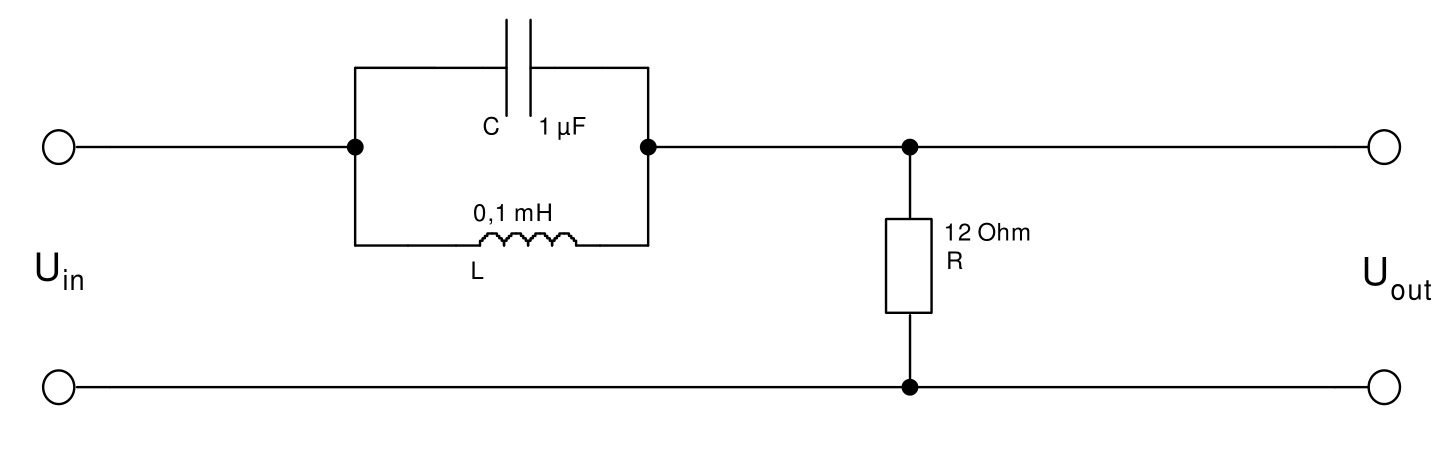
\includegraphics[scale=0.2]{./img/4b_schaltung.png}
    \end{center}
    \end{figure}
    \begin{equation*}
        \frac{U_{out}}{U_{in}}
        =
        \frac{\left\vert Z_R \right\vert}{\left\vert \frac{1}{\frac{1}{Z_C}+\frac{1}{Z_L}}
        +Z_R \right\vert }
        =
        \frac{R}{\sqrt{\left(\frac{\omega L}{\omega^2 C L +1}\right)^2 +
        R^2}}
    \end{equation*}
\end{frame}
\begin{frame}
    \frametitle{Aufgabe 4}
    \framesubtitle{Bode-Diagramm Sperrkreisfilter}
     \begin{figure}[H]
     \begin{center}
             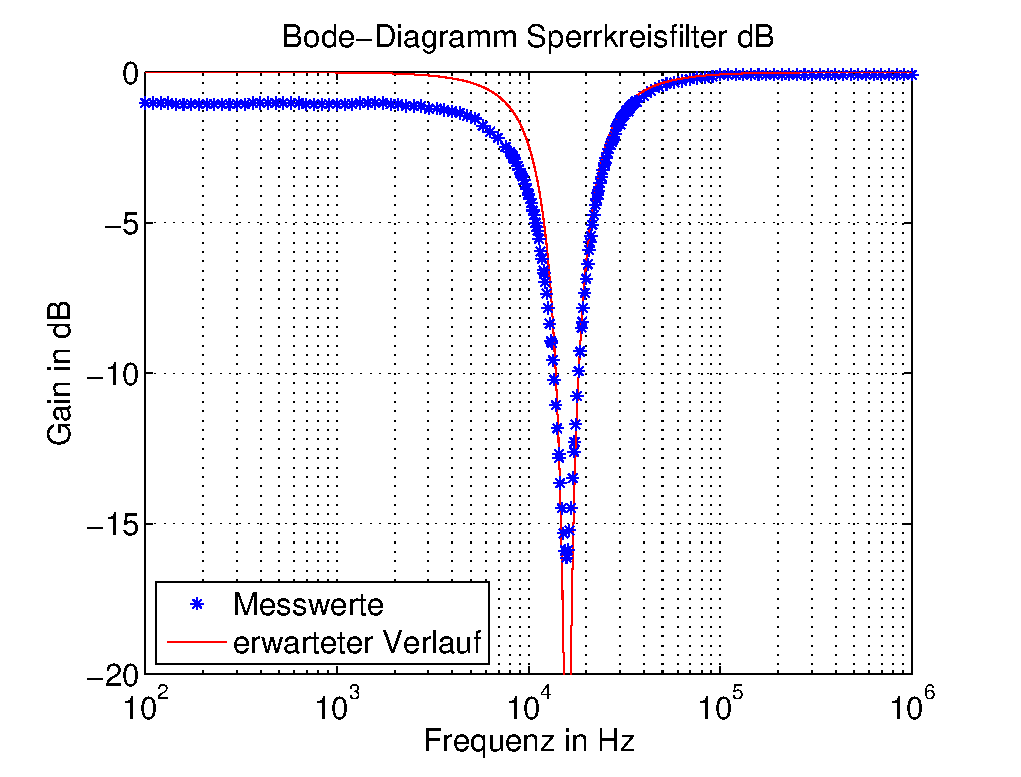
\includegraphics[scale=0.55]{./img/4b_dB.eps}
     \end{center}
     \end{figure}
\end{frame}
\begin{frame}
    \frametitle{Aufgabe 4}
    \framesubtitle{Bode-Diagramm Sperrkreisfilter}
     \begin{figure}[H]
     \begin{center}
             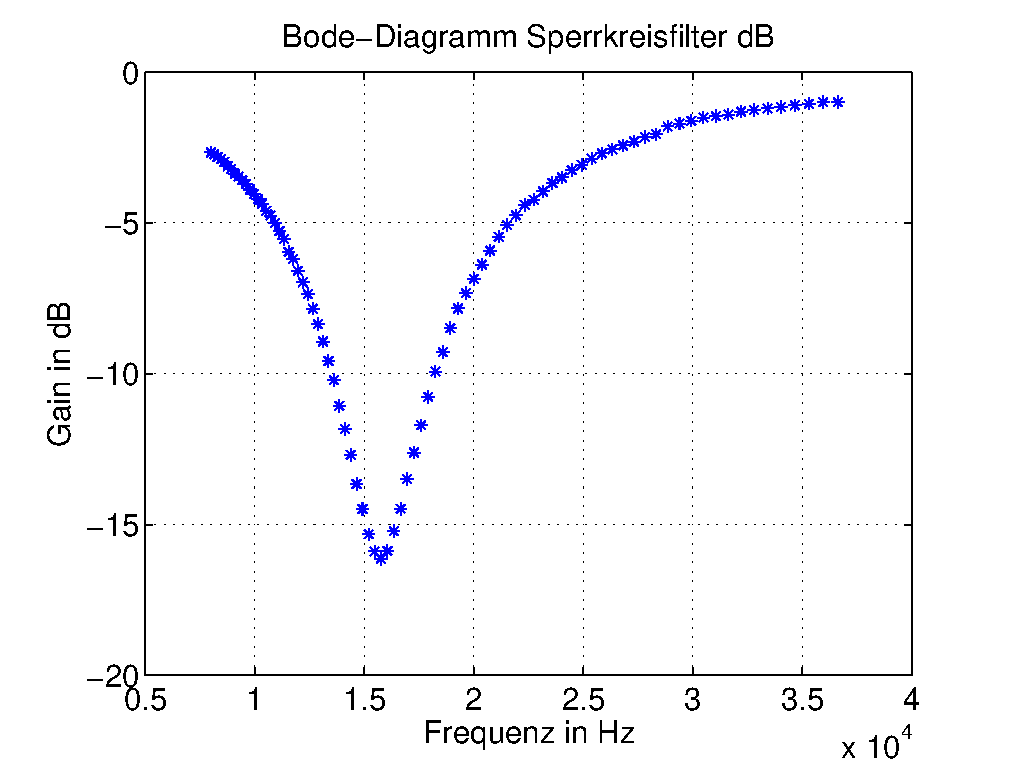
\includegraphics[scale=0.45]{./img/4b_Peak.eps}
     \end{center}
     \end{figure}
    \begin{itemize}
        \item Filtert einzelne Frequenz raus: $f \approx 16 kHz$
        \item Theorie: $f= \frac{1}{2\pi \sqrt{LC}}=15.91kHz$
    \end{itemize}
\end{frame}
\begin{frame}
    \frametitle{Aufgabe 4}
    \framesubtitle{Bode-Diagramm Sperrkreisfilter Phase}
     \begin{figure}[H]
     \begin{center}
             \includegraphics[scale=0.55]{./img/4b_Phase.eps}
     \end{center}
     \end{figure}
     \begin{itemize}
         \item Phase dreht sich beim Peak um
     \end{itemize}
\end{frame}

\begin{frame}
\frametitle{Aufgabe 5a}
\framesubtitle{}
\begin{itemize}
    \item Mit Labview wurden Störfrequenzen in das Signal eingespeist
    \item Analyse der störenden Frequenzen im Oszilloskop
\end{itemize}
Gemessene Störfrequenzen:
\begin{center}
    \begin{tabular}{c|c}
        Gerät & Frequenz/kHz \\
        \hline
        PC & 53.7 \\
        Monitor & 55.0, 66.5 \\
        Oszillosop & 57.3 \\
        DMM & 94.1 \\
        Frequenzgenerator &45.6,60.6 \\
        Kaffeemaschine & keine erkennbaren Frequenzen
    \end{tabular}
\end{center}
\end{frame}

\begin{frame}
\frametitle{Aufgabe 5b}
\framesubtitle{}
    \begin{itemize}
        \item Messung der Störung kleiner Spannungen durch Versuchsgeräte.
        \item Wiederholte Messung bei nähergelegten Kabeln
    \end{itemize}
\end{frame}
\begin{frame}
\frametitle{Aufgabe 5b}
\framesubtitle{}
\begin{center}
    \begin{tabular}{c|c}
        Gerät & Frequenz/kHz \\
        \hline
        Funktionsgenerator & 44.4 , 57,1, 62.3, 82,4, 76.0 \\
        DMM & 57.1 , 81.1 \\
        Monitor& 47.7 , 55.8, 64.2
    \end{tabular}

Mit Koaxialkabel: Keine Störungen. \\
$\rightarrow$  Der räumliche Versuchsaufbau hat Auswirkung auf die Messung \\
$\rightarrow$  Zur exakter Messung Störquellen vom Messort entfernen, oder
Koaxialkabel verwenden \\
$\rightarrow$ Keine unnötigen Geräte betreieben
\end{center}
\end{frame}

    
\end{document}
